% Informe del clasificador de radiografías con Teachable Machine.
\documentclass[a4paper,11pt]{article}

\usepackage[spanish]{babel}
\usepackage[T1]{fontenc}
\usepackage{newpxtext,newpxmath}
\usepackage{microtype}
\usepackage[skip=0.6\baselineskip]{parskip}
\usepackage[a4paper,margin=2.5cm]{geometry}
\usepackage{amsmath}
\usepackage{booktabs}
\usepackage{float}
\usepackage{graphicx}
\usepackage{url}
\usepackage{xcolor}
\usepackage{titlesec}
\usepackage{listings}

\definecolor{editorialink}{HTML}{292927}
\definecolor{editorialaccent}{HTML}{984C3D}
\usepackage[colorlinks=true,linkcolor=editorialaccent,citecolor=editorialaccent,
  urlcolor=editorialaccent,breaklinks=true,pdfauthor={Jheison Martinez Bolivar},
  pdftitle={Clasificador de radiografías de tórax con Teachable Machine}]{hyperref}

\titleformat{\section}{\normalfont\Large\bfseries\color{editorialink}}
{\textcolor{editorialaccent}{\thesection}}{0.75em}{}
\titlespacing*{\section}{0pt}{1.45\baselineskip}{0.55\baselineskip}
\titleformat{\subsection}{\normalfont\large\bfseries\color{editorialink}}
{\thesubsection}{0.7em}{}
\titlespacing*{\subsection}{0pt}{1.15\baselineskip}{0.4\baselineskip}
\setlength{\emergencystretch}{2em}

% Listados de código de los anexos.
\lstset{basicstyle=\ttfamily\footnotesize,numbers=left,numberstyle=\tiny\color{gray},breaklines=true,frame=single,columns=fullflexible,keepspaces=true}

% Captura de pantalla de Teachable Machine, centrada y más compacta.
\newcommand{\figura}[2]{%
  \begin{figure}[H]
    \centering
    \includegraphics[width=0.6\linewidth]{capturas/#1}
    \caption{#2}
  \end{figure}
}

% Dos capturas lado a lado, para ahorrar espacio.
\newcommand{\figuraPar}[4]{%
  \begin{figure}[H]
    \centering
    \begin{minipage}[t]{0.48\linewidth}
      \centering
      \includegraphics[width=\linewidth]{capturas/#1}
      \caption{#2}
    \end{minipage}\hfill
    \begin{minipage}[t]{0.48\linewidth}
      \centering
      \includegraphics[width=\linewidth]{capturas/#3}
      \caption{#4}
    \end{minipage}
  \end{figure}
}

\title{Clasificador de radiografías de tórax con Teachable Machine}
\author{Jheison Martinez Bolivar}
\date{\today}

\begin{document}

  \maketitle

  \begin{abstract}
    Este informe describe el dataset SPR X-Ray Age and Gender, formado por
    radiografías de tórax, y el proceso seguido para entrenar con él un
    clasificador de imágenes sin código en Teachable Machine. Se analizan la
    resolución, los píxeles y la profundidad de color de las imágenes, se
    documentan las corridas de entrenamiento para edad y para género, y se
    prueba el modelo exportado con un script.
  \end{abstract}

  %=========================================================================
  \section{Introducción}
  \subsection{Objetivo}
  Entrenar un modelo de clasificación de imágenes en Teachable
  Machine~\cite{teachable_machine} con radiografías de tórax, caracterizar las
  imágenes del dataset (píxeles, resolución y profundidad de color) y
  documentar el proceso y los resultados.

  \subsection{Descripción del dataset}
  El dataset SPR X-Ray Age and Gender~\cite{kitamura_spr} reúne radiografías de
  tórax de pacientes adultos. Trae 10\,702 imágenes de entrenamiento con dos
  etiquetas por imagen: la edad en años y el género, codificado como 0 o 1. Trae
  además 11\,747 imágenes de prueba sin etiqueta, pensadas para la competencia,
  que no se usan aquí. La licencia es CC BY-NC-ND 4.0: el uso es no comercial y
  los datos no se redistribuyen.

  La edad va de 18 a 89 años, con media de 50.7 y mediana de 48. El género 0 tiene
  6\,209 imágenes (58\,\%) y el 1 tiene 4\,493 (42\,\%). Con la inspección visual
  de las imágenes se asignó el 0 a \textit{mujer} y el 1 a \textit{hombre}.

  El dataset no contiene niños ni adolescentes, porque la edad mínima es 18
  años. Por eso la clasificación por edad usa tres grupos con cortes
  convencionales:

  \begin{table}[H]
    \centering
    \caption{Grupos de edad y número de imágenes disponibles}
    \label{tab:grupos}
    \begin{tabular}{lcc}
      \toprule
      Grupo & Rango de edad & Imágenes disponibles \\
      \midrule
      Joven & 18--29 años & 1\,646 \\
      Adulto & 30--59 años & 5\,067 \\
      Adulto mayor & 60 años o más & 3\,989 \\
      \bottomrule
    \end{tabular}
  \end{table}

  %=========================================================================
  \section{Metodología}
  \subsection{Análisis de las imágenes}
  Las características del dataset se obtienen en dos niveles con el script
  \texttt{08\_analisis\_pixeles.py}. Primero se leen las cabeceras de las 10\,702
  imágenes de entrenamiento (formato, modo de color, tamaño, resolución en dpi y
  programa que generó el archivo). Después se decodifican los píxeles de una
  muestra aleatoria de 500 imágenes, con semilla fija, y se calculan canales,
  igualdad entre canales, canal alfa, valores únicos, media, desviación,
  percentiles, fracción de píxeles negros y blancos e histograma de intensidad.

  \subsection{Muestras}
  Las muestras para Teachable Machine se toman al azar con semilla fija, para que
  se puedan reproducir. Las imágenes de prueba nunca se usan para entrenar, y
  las de entrenamiento de cada tarea tampoco se mezclan con las de prueba.

  \begin{table}[H]
    \centering
    \caption{Muestras usadas en cada corrida}
    \label{tab:muestras}
    \begin{tabular}{llcc}
      \toprule
      Tarea & Conjunto & Imágenes por clase & Script \\
      \midrule
      Edad & Entrenamiento & 200 y después 600 & \texttt{04\_muestra\_edad.py} \\
      Edad & Prueba & 10 & \texttt{05\_prueba.py} \\
      Género & Entrenamiento & 600 & \texttt{06\_muestra\_genero.py} \\
      Género & Prueba & 10 & \texttt{06\_muestra\_genero.py} \\
      \bottomrule
    \end{tabular}
  \end{table}

  \subsection{Proceso en Teachable Machine}
  El proceso en la herramienta web sigue estos pasos:
  \begin{enumerate}
    \item Crear un proyecto de imágenes y definir una clase por categoría. Para
      edad son \textit{Joven}, \textit{Adulto} y \textit{Adulto Mayor}; para
      género son \textit{Female} y \textit{Male}.
    \item Cargar las imágenes de cada clase con el botón \textit{Subir},
      seleccionando los archivos de la carpeta correspondiente.
    \item Abrir la opción \textit{Avanzado} y fijar épocas, tamaño del lote y
      tasa de aprendizaje. Los valores por defecto son 50, 16 y 0.001.
    \item Pulsar \textit{Preparar modelo} y esperar a que termine el
      entrenamiento.
    \item Probar el modelo en la vista previa con entrada \textit{Archivo},
      subiendo radiografías que no se usaron para entrenar.
    \item Exportar el modelo con \textit{Exportar modelo}, en formato
      TensorFlow/Keras. El zip resultante contiene el modelo y las etiquetas
      de las clases, y se prueba con un script en Python.
  \end{enumerate}

  \subsection{Corridas de entrenamiento}
  \subsubsection*{Edad, 200 imágenes por clase, valores por defecto}
  Se cargan las tres clases con 200 imágenes cada una y se entrena con 50
  épocas, lote de 16 y tasa de aprendizaje de 0.001.

  \figuraPar{01-cargando-imagenes.png}{Tres clases de edad con 200 imágenes cada una}{02-entrenando-50-epocas.png}{Entrenamiento con 50 épocas, lote 16 y tasa 0.001}

  \subsubsection*{Edad, 100 épocas}
  Se sube solo el número de épocas a 100 y se mantienen el lote y la tasa.

  \figura{08-reentrenando-100-epocas.png}{Reentrenamiento con 100 épocas en curso}

  \subsubsection*{Edad, 600 imágenes por clase, valores por defecto}
  Se repite el entrenamiento por defecto con 600 imágenes por clase.

  \figura{07-entrenando-600-default.png}{Entrenamiento con 600 imágenes por clase y valores por defecto}

  \subsubsection*{Género, 600 imágenes por clase, valores por defecto}
  Se pasa a género porque la etiqueta viene directamente en el dataset y sirve
  para comparar con el ejercicio de edad. Teachable Machine llama a las clases
  \textit{Female} y \textit{Male}.

  \figura{09-entrenando-genero.png}{Entrenamiento de género con 600 imágenes por clase y valores por defecto}

  \subsection{Prueba automática del modelo exportado}
  El script \texttt{07\_probar\_modelo.py} carga el modelo exportado y lo prueba
  sobre las imágenes de \texttt{data/prueba\_genero}: 10 por clase, que no se
  usaron para entrenar. Su preprocesamiento replica el de Teachable Machine:
  ajustar a 224 $\times$ 224 con recorte central y normalizar a $[-1, 1]$. El
  modelo se carga y se consulta una imagen a la vez.

  \begin{code}[lang=python]
def preparar(ruta_imagen):
    imagen = Image.open(ruta_imagen).convert("RGB")
    imagen = ImageOps.fit(imagen, TAMANO, Image.Resampling.LANCZOS)
    arreglo = np.asarray(imagen).astype(np.float32) / 127.5 - 1
    return arreglo

modelo = tf.keras.models.load_model(carpeta_modelo / "keras_model.h5", compile=False)
etiquetas = cargar_etiquetas(carpeta_modelo / "labels.txt")

for imagen in imagenes:
    entrada = np.expand_dims(preparar(imagen), axis=0)
    probabilidades = modelo.predict(entrada, verbose=0)[0]
    indice = int(np.argmax(probabilidades))
    predicha = etiquetas[indice]
    acierto = predicha == esperada
  \end{code}

  %=========================================================================
  \section{Resultados}
  \subsection{Características del dataset}
  \subsubsection*{Resolución y formato}
  Las 10\,702 imágenes de entrenamiento tienen el mismo tamaño: \textbf{1024
  $\times$ 1024 píxeles}, es decir, 1\,048\,576 píxeles por imagen, todas
  cuadradas y en formato PNG, que comprime sin pérdida. El tamaño promedio por
  archivo es de 756 KB y el conjunto de entrenamiento ocupa 8.1 GB. No hay
  imágenes de otro tamaño, así que no hace falta unificar la resolución antes de
  entrenar.

  \subsubsection*{Descripción de los píxeles}
  Cada píxel tiene cuatro canales: rojo, verde, azul y alfa. La Cuadro~\ref{tab:pixeles}
  resume una muestra aleatoria de 500 imágenes.

  \begin{table}[H]
    \centering
    \caption{Características de los píxeles en una muestra de 500 imágenes}
    \label{tab:pixeles}
    \begin{tabular}{ll}
      \toprule
      Característica & Resultado \\
      \midrule
      Modo de color (Pillow) & RGBA \\
      Canales por píxel & 4 (R, G, B, alfa) \\
      Bits por canal & 8 (valores de 0 a 255) \\
      Canal alfa & 255 en todos los píxeles (imagen opaca) \\
      R, G y B iguales & Sí, en las 500 imágenes \\
      Valores únicos en el canal R & Mediana 233; mínimo 185; máximo 256 \\
      Intensidad media & 126.7 (de 0 a 255) \\
      Desviación estándar media & 53.3 \\
      Percentiles 1, 50 y 99 & 28.8, 133.8 y 205.7 \\
      Píxeles negros (valor 0) & 2.32\,\% \\
      Píxeles blancos (valor 255) & 0.00\,\% \\
      \bottomrule
    \end{tabular}
  \end{table}

  La Figura~\ref{fig:histograma} muestra una radiografía de ejemplo y el
  histograma de intensidad de las 500 imágenes. El histograma tiene un pico en 0,
  que corresponde a los bordes y fondos negros (2.32\,\% de los píxeles), un
  grupo de valores entre 30 y 55, y una distribución amplia que sube hasta cerca
  de 175 y cae hacia 215. Ningún píxel llega a 255 y el percentil 99 es 205.7, así
  que las imágenes no usan el extremo superior de la escala: el contraste no
  está estirado a todo el rango.

  \begin{figure}[H]
    \centering
    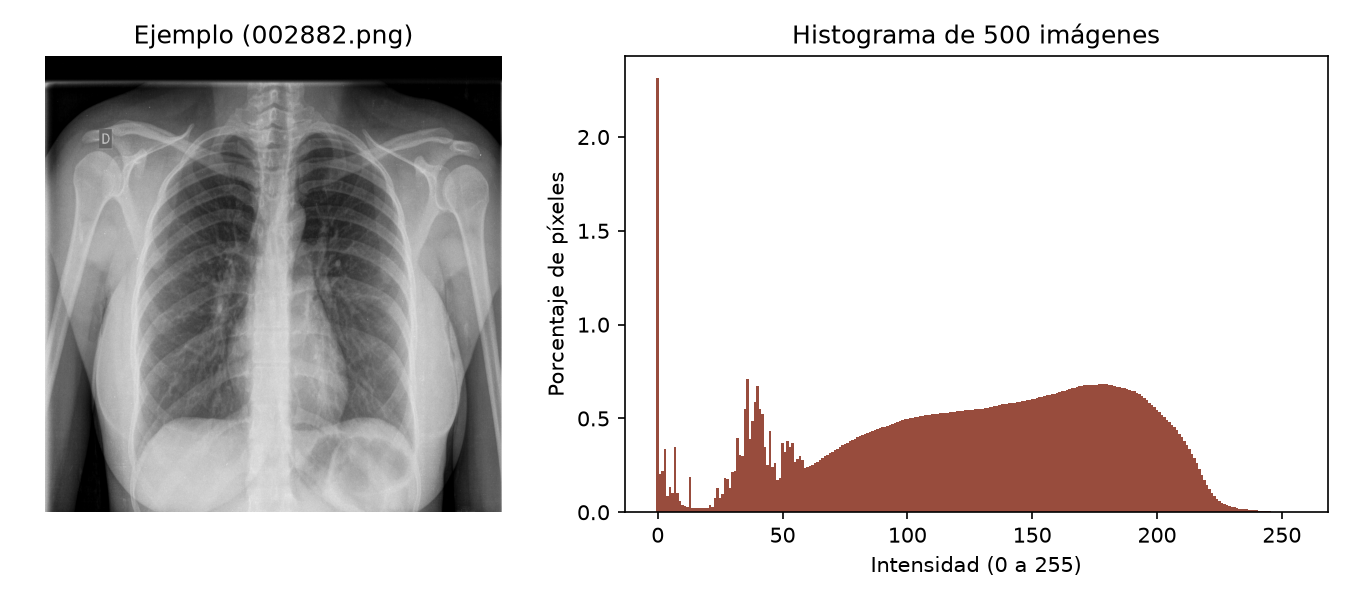
\includegraphics[width=\linewidth]{figuras/ejemplo_histograma.png}
    \caption{Radiografía de ejemplo e histograma de intensidad de 500 imágenes}
    \label{fig:histograma}
  \end{figure}

  \subsubsection*{Profundidad de color}
  Cada canal usa 8 bits, así que cada píxel ocupa 32 bits y una imagen sin
  comprimir ocuparía 4 MiB. Sin embargo, la imagen es en escala de grises
  guardada como RGB: R, G y B son iguales en todas las muestras. La información
  real es un solo canal de 8 bits (256 niveles de gris), es decir, 1 MiB. El
  canal alfa no aporta nada, porque vale 255 en todos los píxeles. De los 32 bits
  por píxel, solo 8 llevan información.

  Las imágenes no aprovechan los 256 niveles: la mediana de valores distintos por
  imagen es 233 y en alguna imagen hay solo 185. La compresión PNG compensa el
  espacio redundante: el archivo promedio pesa 0.72 MiB, unas 5.6 veces menos
  que los 4 MiB sin comprimir.

  Teachable Machine convierte cada imagen a RGB de 224 $\times$ 224 píxeles
  antes de entrenar. Eso reduce cada lado en un factor de 4.6 y deja el 4.8\,\%
  de los píxeles originales (50\,176 de 1\,048\,576). La imagen de entrada del
  modelo tiene $224 \times 224 \times 3 = 150\,528$ valores, y los tres canales
  siguen siendo iguales, porque la imagen original ya era de grises.

  \subsubsection*{Origen de las imágenes}
  Los metadatos de los PNG indican que todos se escribieron con Matplotlib
  (versión 3.4.1 en 7\,655 imágenes y 3.7.0 en 3\,047) y con una resolución
  declarada de 100 dpi. Eso sugiere que no son las radiografías originales, sino
  renderizados a 8 bits hechos para el dataset. Con estos archivos no se puede
  saber cuál era la profundidad de bits de las imágenes de origen.

  \subsection{Resultados de los modelos de edad}
  Con 200 imágenes por clase y los valores por defecto, una radiografía de la
  clase adulto da 91\,\% para adulto. Con otra imagen, que se consideró mal
  etiquetada, el modelo dio 71\,\% para joven y 29\,\% para adulto.

  \figuraPar{03-adulto-bien-etiquetado.png}{Radiografía de adulto: 91\,\% para adulto}{04-adulto-mal-etiquetado.png}{Radiografía de una clase distinta: 71\,\% para joven}

  Con 100 épocas el modelo queda seguro de sus respuestas: en algunas imágenes da
  100\,\% a una clase, y en una de ellas el resultado no coincide con lo
  esperado.

  \figuraPar{05-etiquetas-fuertes-100-epocas.png}{100 épocas: 100\,\% para adulto en una radiografía}{06-100-porciento-equivocado.png}{100 épocas: 100\,\% para adulto mayor en una radiografía que resultó equivocada}

  Con 600 imágenes por clase y los valores por defecto, los resultados fueron
  prácticamente los mismos que con 200. Cambiar el número de épocas o de
  imágenes no mejoró el modelo de forma visible. Con 30 imágenes de prueba, una
  diferencia de uno o dos aciertos no alcanza para concluir nada.

  \subsection{Resultados del modelo de género}
  \subsubsection*{Pruebas en la web}
  Las pruebas se hicieron subiendo radiografías a la vista previa de Teachable
  Machine. La mayoría de las pruebas dieron la clase correcta. Una falló: la
  imagen \texttt{010335.png}, de la clase \textit{mujer} (etiqueta 0 del
  dataset), se clasificó como \textit{hombre}. Esa imagen no estaba en ninguna
  muestra del proyecto.

  % Completar con las pruebas web que salieron bien y las capturas de cada una.

  \subsubsection*{Prueba automática sobre 20 imágenes}
  El modelo exportado acierta 18 de 20 (90\,\%): 9 de 10 mujeres y 9 de 10
  hombres. Los dos errores son \texttt{010335.png} (mujer, predicha como hombre,
  confianza 83\,\%) y \texttt{008368.png} (hombre, predicha como mujer, confianza
  98\,\%). La Cuadro~\ref{tab:resumen} resume los aciertos por clase y la
  Cuadro~\ref{tab:imagenes} muestra la predicción de cada imagen.

  \begin{table}[H]
    \centering
    \caption{Aciertos por clase en la prueba de género}
    \label{tab:resumen}
    \begin{tabular}{lccc}
      \toprule
      Clase esperada & Aciertos & Total & Porcentaje \\
      \midrule
      Female (mujer) & 9 & 10 & 90\,\% \\
      Male (hombre) & 9 & 10 & 90\,\% \\
      \midrule
      Total & 18 & 20 & 90\,\% \\
      \bottomrule
    \end{tabular}
  \end{table}

  \begin{table}[H]
    \centering
    \small
    \caption{Predicción de cada imagen de prueba (\texttt{resultados/genero.csv})}
    \label{tab:imagenes}
    \begin{tabular}{llllc}
      \toprule
      Archivo & Esperada & Predicha & Confianza & Acierto \\
      \midrule
      hombre/001647.png & Male & Male & 87.62\,\% & Sí \\
      hombre/003046.png & Male & Male & 99.92\,\% & Sí \\
      hombre/003495.png & Male & Male & 100.00\,\% & Sí \\
      hombre/004239.png & Male & Male & 99.60\,\% & Sí \\
      hombre/005507.png & Male & Male & 99.99\,\% & Sí \\
      hombre/006466.png & Male & Male & 100.00\,\% & Sí \\
      hombre/007026.png & Male & Male & 100.00\,\% & Sí \\
      hombre/007058.png & Male & Male & 100.00\,\% & Sí \\
      hombre/008368.png & Male & Female & 98.17\,\% & No \\
      hombre/010001.png & Male & Male & 52.66\,\% & Sí \\
      mujer/000212.png & Female & Female & 99.96\,\% & Sí \\
      mujer/000568.png & Female & Female & 96.17\,\% & Sí \\
      mujer/002003.png & Female & Female & 100.00\,\% & Sí \\
      mujer/002100.png & Female & Female & 99.77\,\% & Sí \\
      mujer/007036.png & Female & Female & 99.96\,\% & Sí \\
      mujer/008923.png & Female & Female & 100.00\,\% & Sí \\
      mujer/008967.png & Female & Female & 99.44\,\% & Sí \\
      mujer/009916.png & Female & Female & 100.00\,\% & Sí \\
      mujer/010072.png & Female & Female & 100.00\,\% & Sí \\
      mujer/010335.png & Female & Male & 83.46\,\% & No \\
      \bottomrule
    \end{tabular}
  \end{table}

  Al terminar, el script imprime en consola el resumen de la corrida:

  \begin{code}[lang=text]
Female      9   10
Male        9   10
Total: 18 de 20 correctas
  \end{code}

  %=========================================================================
  \section{Conclusiones}
  \subsection{Sobre las características de las imágenes}
  \begin{itemize}
    \item Las 10\,702 imágenes de entrenamiento son homogéneas: todas son
      PNG de 1024 $\times$ 1024 píxeles, así que no hace falta unificar el
      tamaño.
    \item Las imágenes son de escala de grises (R = G = B) guardadas en modo
      RGBA. La información real es de un solo canal de 8 bits; los otros 24 bits
      por píxel son redundantes (dos canales repetidos y un alfa constante).
    \item Las imágenes no usan todo el rango de intensidad: no hay píxeles en
      255, el percentil 99 es 205.7 y hay entre 185 y 256 niveles distintos por
      imagen. Hay un 2.3\,\% de píxeles negros, que corresponden a bordes.
    \item Los metadatos indican que los PNG se generaron con Matplotlib. Son
      renderizados a 8 bits, y no se puede saber la profundidad de color de las
      radiografías originales.
    \item Teachable Machine reduce las imágenes a 224 $\times$ 224 y las convierte
      a RGB, con lo que conserva solo el 4.8\,\% de los píxeles. Los detalles
      finos de las radiografías se pierden en esa reducción.
  \end{itemize}

  \subsection{Sobre los modelos}
  La clasificación por edad no mostró una mejora clara al cambiar épocas o
  tamaño de la muestra. La clasificación por género dio 18 de 20 aciertos sobre
  imágenes que no se usaron para entrenar.

  \subsection{Limitaciones}
  El tamaño de las pruebas (20 imágenes para género y 30 para edad) no permite
  distinguir diferencias pequeñas. Además, las etiquetas de edad y género del
  dataset no se verificaron de forma independiente. El paso siguiente sería una
  prueba más grande y, para edad, revisar los grupos con más imágenes.

  \bibliographystyle{plain}
  \bibliography{bib/references}

  \appendix
  \section{Anexo: script de prueba del modelo}
  Listado completo de \texttt{scripts/07\_probar\_modelo.py}, que carga el modelo
  exportado de Teachable Machine y lo prueba sobre una carpeta de imágenes.

  \lstinputlisting[language=Python]{anexos/07_probar_modelo.py}

\end{document}
